\section{Limitations} \label{sec:limitations}
In this section we will present the main limitation of the developed system, mainly in the software components.
Most of these limitations exist due to development choices and not due to any particular impediment from realising them.
The main reasons that led us to make such choices include, but are not limited to, the project development being done by a single person, limited development time and, most importantly, the fact that the entire project has been developed from a home environment during the Portuguese COVID-19 lock-downs in early 2021.

% Hardware
\subsection{Hardware}
For the most part, the hardware components were chosen in a way they would not pose a big obstacle to the development of more advanced demonstration concepts.
Regardless, the designed and 3D-printed motor support was mostly meant to allow the motor to function properly without the user having to hold on to it.

This was one of the limitations that rose from developing the project from a home environment, where the development of the 3D model had to be done in an open-loop situation, without any feedback or preliminary testing before sending the complete design for production.
Ultimately this meant one of the 3D printed pieces was defective but, luckily, the problem was lessened with some hot glue, as seen in \autoref{fig:hotglue-support} (page \pageref{fig:hotglue-support}).

\begin{figure}[t]
	\centering
	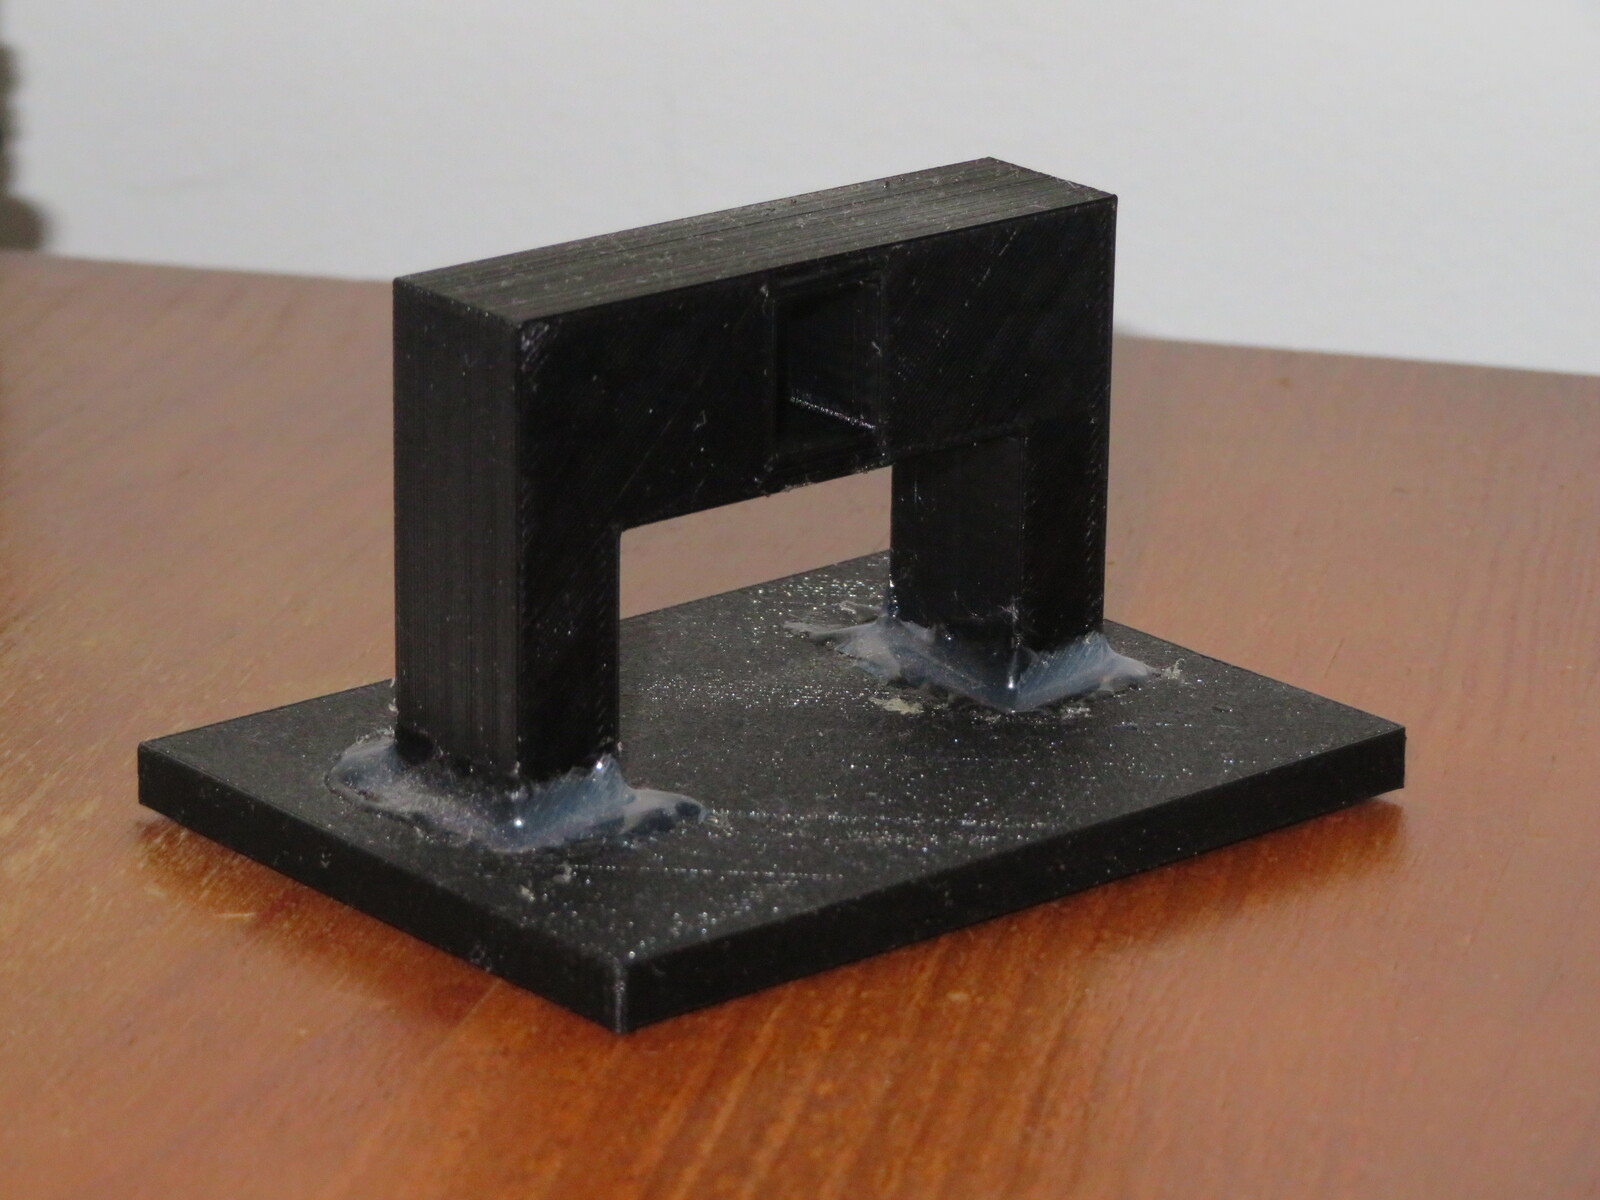
\includegraphics[width=0.8\linewidth]{IMG_3044_resized.JPG}
	\caption{3D printed support, fixed with hot glue}
	\label{fig:hotglue-support}
\end{figure}

Another hardware aspect that could be considered a limitation is the small encoder resolution (12 PPR).
This has not impacted the performance because the motor's gearbox, with a reduction ratio of $30:1$, makes the motor + gearbox + encoder set have an apparent 360 PPR encoder on the output shaft.
As we are only interested in controlling said output shaft, the actual (virtual) encoder resolution is more than enough for a proof-of-concept system.

% Comm
% Limited I/O bytes
% Not using the remote synchronise feature
\subsection{netHAT 52-RTE driver}
Although the other RTE networks supported by the netHAT 52-RTE board should work out-of-the-box with the developed handler, they have not been tested.
Therefore, the current implementation for said handler could be limited to only working with the EtherCAT protocol, which is the only one properly tested.

First of all, EtherCAT includes a remote synchronisation feature that allows the master device to send a \verb|sync| command which will make all slaves update the outputs at the same time.
This feature is supported by the Hilscher's netHAT driver but it has not been included on the developed handler library.
We did not dedicate time to add support for this feature as the designed system would not use it.
Furthermore, we acknowledge that more advanced demonstration concepts would definitely benefit from utilising such feature, especially the ones that would use multiple slave devices simultaneously.
Regardless, the documentation on the netHAT CIFX API states that `Fieldbus synchronization must be supported by the used fieldbus protocol stack.' \cite{nethat:cifx_api_docs}, meaning such feature will only work if the underlying RTE protocol supports it.

One more characteristic that may pose a limitation, mostly on larger and more complex demonstration concepts, is the fixed-size cyclic Input/Output (I/O) data.
As mentioned previously, the netHAT 52-RTE board provides 32 bytes for each input and output cyclic data types.
Although this amount of data is more than sufficient for our proof-of-concept system, it might not be adequate for more advanced case scenarios.

% Encoder (SW)
\subsection{Encoder interface}
By the end of the development phase of this project, the encoder interface used and the driver implemented were very targeted for the specific model we used.
The electrical connection only supports Transistor-Transistor Logic (TTL) signals up to $3.3V$ and does not support differential signals \cite{technology:diff-signals}, due to the direct connection with the Raspberry Pi's GPIO pins.
Although this was the planned way of implementing such interface, one can utilise an external logic processing unit to convert differential signals to absolute ones, which can then replace the current electrical connections.

Furthermore, as the encoder used on our project did not include an Index output (one short pulse every revolution), we did not add support for it on the developed driver.
Effectively, no mechanism for `homing' the absolute position of the motor was implemented, because it was also out of the scope for the current project.

% PV calc
% `- Fixed period instead of fixed inputs - more complicated to implement due to callback from libgpiod
\subsection{Velocity calculation}
The current implementation of the velocity calculation uses an algorithm based on a fixed time period.
The algorithm takes into account how many encoder pulses have been acquired over the time period, using the encoder counter, and calculates the velocity based on its fixed period.
This had the advantage of being simple to implement, but for applications that require precise measurements, it is not the best option.
At low speeds, this algorithm has poor precision, including a gap between measuring a speed of 0 and whichever speed corresponds to exactly one encoder pulse per iteration of the calculation algorithm.

One possible improvement is to design and implement an algorithm based on a dynamic period that uses an interrupt-driven logic.
Every time a new encoder pulse is detected, an interrupt is generated which triggers the velocity calculation.
This algorithm is based on measuring how much time is elapsed between consecutive encoder pulses and provides far better precision at low speeds, as well as possibly reduced CPU usage, especially during such cases.
It would still be necessary to determine a timeout period of when to consider a null velocity, but that would still be way more flexible than the current implementation, which indirectly controls said timeout through the desired cycle period.
It has been determined that the \verb|libgpiod| library in use is capable of calling a function whenever an input changes its state (callback method), so implementing this other algorithm should be doable without the need to introduce new libraries.

% Main
% `- parameters can only be passed via command-line arguments, no configuration file is supported
When it comes to user friendliness, the main launcher of the application could have been a bit more polished.
This was mostly due to the limited time period for development, but all the necessary features were still achieved.

For simplicity reasons we only implemented a single way of providing the control application the necessary parameters: command-line arguments.
We had planned on implementing some form of configuration file which would hold the necessary parameter values, but we ended up not implementing it.
Instead, a wrapper-launcher can be written which stores the command-line argument values. For example a \verb|bash| script can automatically launch the application with pre-determined values.
A single text file called \verb|run.sh| containing the command shown in \autoref{lst:main-sh} has achieved the goal of storing pre-defined parameter values, so we did not pursue any further options.

\lstinputlisting[float=t,language=bash,label=lst:main-sh,caption=Wrapper script to launch application with pre-defined parameters]{../src/main/run.sh}
